\section{Техническое задание}
\subsection{Основание для разработки}

Основанием для разработки является задание для курсовой работы по предмету   "<Проектирование и архитектура программных систем">.

\subsection{Цель и назначение разработки}

Основной задачей курсовой работы является разработка игры в жанре платформер на языке Python.

Основной целью данной работы является изучение проектирования и архитектуры программных систем на примере игры в жанре платформер.

Задачами данной разработки являются:
\begin{itemize}
\item создание игровых уровней и переход между ними;
\item реализация движения персонажа, включая взаимодействие с различными игровыми объектами;
\item создание системы управления клавишами;
\item тестирование и отладка игры для выявления и устранения ошибок и недоразумений.
\end{itemize}

\subsection{Требования к игре}
\begin{itemize}
\item Список из разных уровней;
\item Уровни, состоящие из тайлов и  различных игровых объектов;
\item Игровой персонаж, которым можно управлять с помощью кнопок клавиатуры;
\item Обработка взаимодействий персонажа с объектами, из которых состоят  уровни.
\end{itemize}

\subsection{Требования пользователя к интерфейсу игры}

Игра должна включать в себя:
\begin{itemize}
    \item Разнообразие игровых уровней с различными типами препятствий и врагов;
    \item Простое и интуитивное управление, позволяющее игрокам наслаждаться игрой без излишних сложностей;
    \item Стильная и детализированная графика, отвечающая атмосфере ретро-игр.
\end{itemize}

Композиция шаблона игры представлена на рисунке ~\ref{fig:maket1}.

\begin{figure}[H]
	\centering
	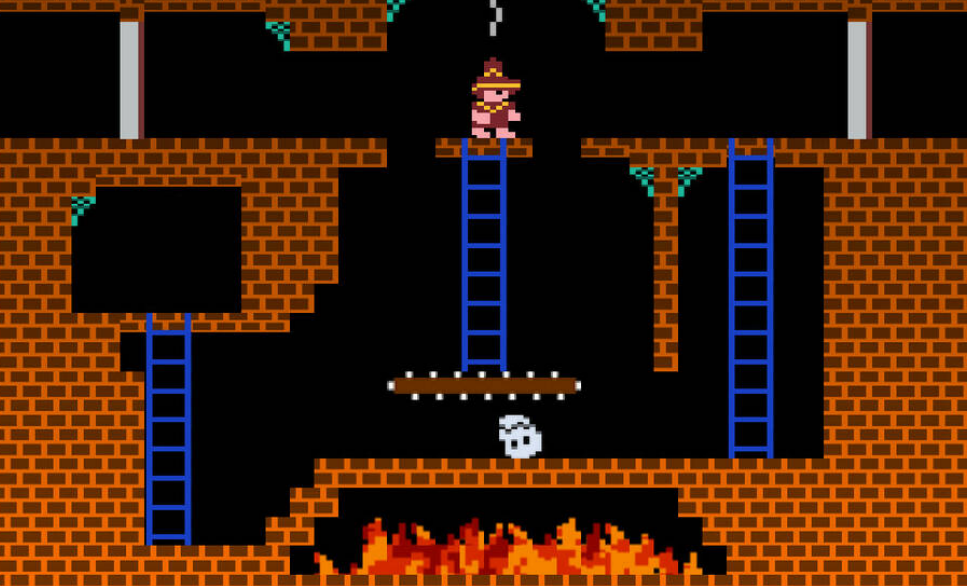
\includegraphics[width=0.9\linewidth]{images/maket1}
	\caption{Композиция шаблона уровня игры}
	\label{fig:maket1}
\end{figure}

%\begin{figure}[ht]
%\caption{Композиция шаблона сайта}
%\label{templ:image}
%\end{figure}
%\vspace{-\figureaboveskip} % двойной отступ не нужен (можно использовать, если раздел заканчивается картинкой)

\subsection{Моделирование вариантов использования}

Для разрабатываемой игры была реализована модель, которая обеспечивает наглядное представление вариантов использования игры.

Она помогает в физической разработке и детальном анализе взаимосвязей объектов. При построении диаграммы вариантов использования применяется унифицированный язык визуального моделирования UML.

На основании анализа предметной области в программе должны быть реализованы следующие прецеденты:
\begin{enumerate}
\item Начать игру.
\item Управление персонажем.
\item Переключение уровней.
\item Взаимодействие с игровыми объектами.
\item Завершение игры.
\end{enumerate}

\begin{figure}[ht]
	\center{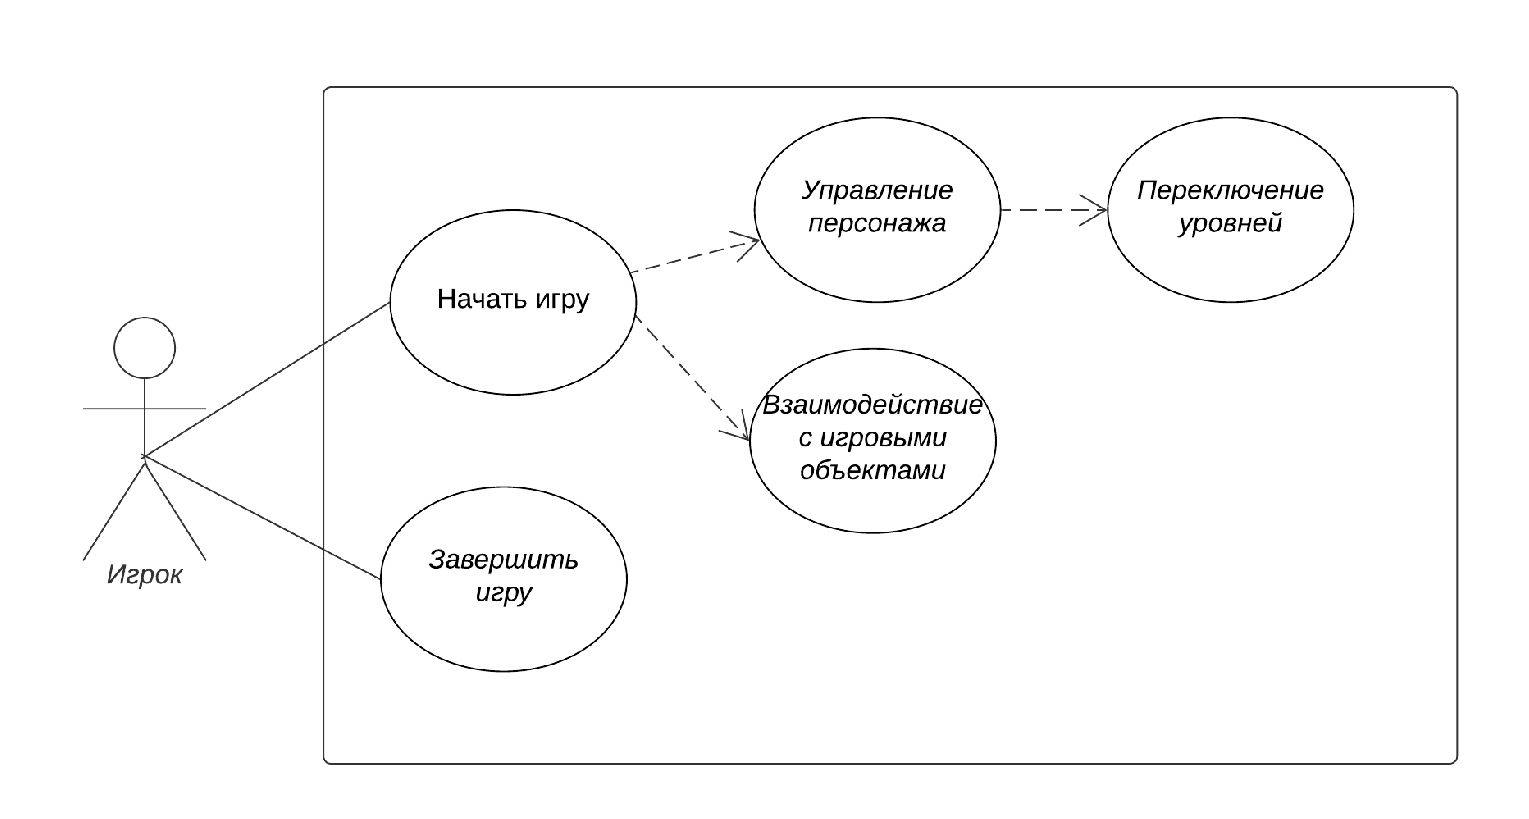
\includegraphics[width=1\linewidth]{precend}}
	\caption{Диаграмма прецедентов}
	\label{precend:image}
\end{figure}

\subsection{Требования к оформлению документации}

Разработка программной документации и программного изделия должна производиться согласно ГОСТ 19.102-77 и ГОСТ 34.601-90. Единая система программной документации.
